\documentclass[svgnames]{beamer}
\mode<presentation>
\usefonttheme{serif}
\usecolortheme{dove}
\useinnertheme{rounded}
%\useoutertheme{smoothbars}
\setbeamercolor{item projected}{fg=black}
\setbeamertemplate{navigation symbols}{}

\usepackage{times}
\usepackage[french]{babel}
\usepackage{amsthm,amssymb,amsmath,graphicx}
\usepackage{color}
\usepackage{gastex}
\usepackage{framed}
\usepackage{graphicx}
\usepackage{multicol}
\usepackage{ulem}
\usepackage{ifthen}
\usepackage{tikz}
\usepackage{appendixnumberbeamer}
\usepackage{eurosym}

%%%%%%%%%%%%%%%%%%%%%%%%%%%%%%%%%%%%%%%%%%%%%%%%%%%%%%%%%%%%%%%%%%%%%%%%%%%%%%%%%%%%%%%%
%%%%%%%%%%%%%%%%%%%% A non-original creation by Nathanaël Fijalkow and Victor Marsault %

\setbeamertemplate{frametitle}{
  \vskip-2pt
  \begin{beamercolorbox}[rightskip=2cm,leftskip=1em,dp=1ex,wd=12.8cm]{frametitle}
    \vskip2pt
    \usebeamercolor{frametitle}
    \begin{tikzpicture}
      \useasboundingbox (0,0) rectangle (0,0); 
      \ifthenelse{\insertframenumber<\inserttotalframenumber}
      { 
        \pgfmathsetmacro{\aimangle}{90-(\insertframenumber*360/\inserttotalframenumber)}
        \fill [fill=frametitle.fg,thin, color=gray!50,draw=black] (11.8,.2) -- (11.8,.6) arc (90:\aimangle:0.4) -- cycle;

      }{ 
        \fill[fill=frametitle.fg,thin, color=gray!50,draw=black] (11.8,0.2) circle (.4);
      }
      \fill[fill=frametitle.fg,thin, color=white,draw=black] (11.8,0.2) circle (.3);
      \node at (11.8, .2) [black,circle]{\normalsize\insertframenumber};
    \end{tikzpicture}
    \insertframetitle
    \vskip2pt
  \end{beamercolorbox}
}
%%%%%%%%%%%%%%%%%%%%%%%%%%%%%%%%%%%%%%%%%%%%%%%%%%%%%%%%%%%%%%%%%%%%%%%%%%%%%%%%%%%%%%%

\setbeamertemplate{blocks}[rounded]
\setbeamercolor{block title}{bg=normal text.bg!90!black}
\setbeamercolor{block body}{bg=normal text.bg!95!black}

\newcommand{\A}{\mathcal{A}}
\newcommand{\Q}{\mathbb{Q}}
\newcommand{\N}{\mathbb{N}}
\newcommand{\tr}[1]{\langle #1 \rangle}
\newcommand{\prob}[1]{\mathbb{P}_{#1}}
\newcommand{\set}[1]{\{ #1 \}}
\newcommand{\val}[1]{\text{val}(#1)}

  
\title{
Momentum 2018 \\
Relever les d{\'e}fis de l'apprentissage automatique
\vskip2em
\textbf{Deep Synthesis} \\
\textit{Apprentissage pour la Synth{\`e}se de Programmes}
}
\subtitle{Nathana{\"e}l Fijalkow}
\institute{

\includegraphics[height=3cm]{Fig/CNRS}
\hspace*{1cm}

\includegraphics[height=3cm]{Fig/LaBRI}
\hspace*{1cm}

\includegraphics[height=3cm]{Fig/Turing}
}
\date{}

\begin{document}

\addtocounter{framenumber}{-1}

\begin{frame}
  \titlepage
\end{frame}

\begin{frame}{Pr{\'e}sentation}

\begin{footnotesize}
\begin{itemize}
	\item Sept. 2008 - Ao{\^u}t 2012 : {\'E}NS Cachan, cursus informatique et math{\'e}matiques
	\item Sept. 2012 - Oct. 2015 : Th{\`e}se cotutelle Paris Diderot - Varsovie
	\item Nov. 2015 - Juill. 2016 : Post-doctorat {\`a} Oxford
	\item Ao{\^u}t 2016 - D{\'e}c. 2016 : Research Fellow au Simons Institute {\`a} Berkeley
\end{itemize}
\end{footnotesize}

\begin{itemize}
	\item depuis Jan. 2017 : \textcolor{red}{Chercheur associ{\'e} au Alan Turing Institute of data science and artificial intelligence} {\`a} Londres, responsable du groupe ``\textcolor{magenta}{fondations logiques des sciences des donn{\'e}es}''
	\item depuis Jan. 2018 : \textcolor{blue}{Charg{\'e} de recherche au CNRS} affili{\'e} au LaBRI, Bordeaux
\end{itemize}

\begin{framed}
\textbf{Discipline {\'e}mergente} : Logic and Learning
\end{framed}
\textbf{En 2018} : \begin{small}organisation de workshop, {\'e}cole de recherche, et ``\textit{Summit on Formal Methods Meets Machine Learning}''\end{small}
\end{frame}

\begin{frame}{Qu'est-ce que la synth{\`e}se (en m{\'e}thodes formelles) ?}

La \textcolor{magenta}{synth{\`e}se} est une proc{\'e}dure :
\begin{itemize}
	\item \textbf{Entr{\'e}e} : \textcolor{red}{sp{\'e}cification} (compl{\`e}te ou partielle)
	\item \textbf{Sortie} : un \textcolor{blue}{syst{\`e}me} r{\'e}alisant la sp{\'e}cification
\end{itemize}

\vskip1em
Trois types de syst{\`e}mes :

\begin{center}
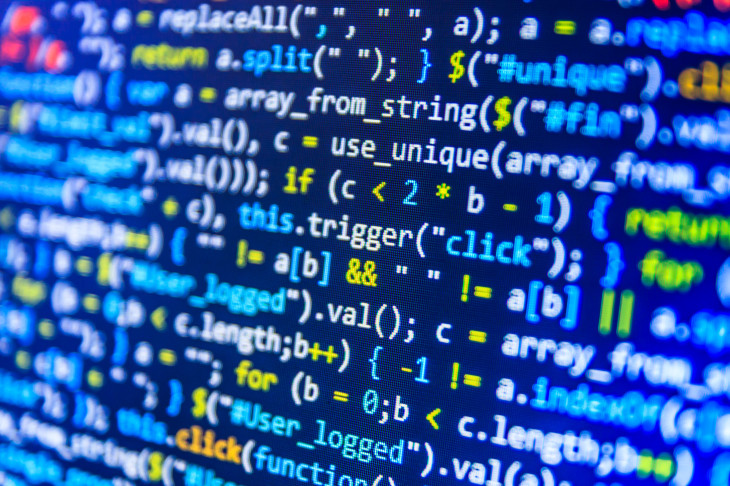
\includegraphics[height=2.5cm]{Fig/code}
\hspace*{.2cm}
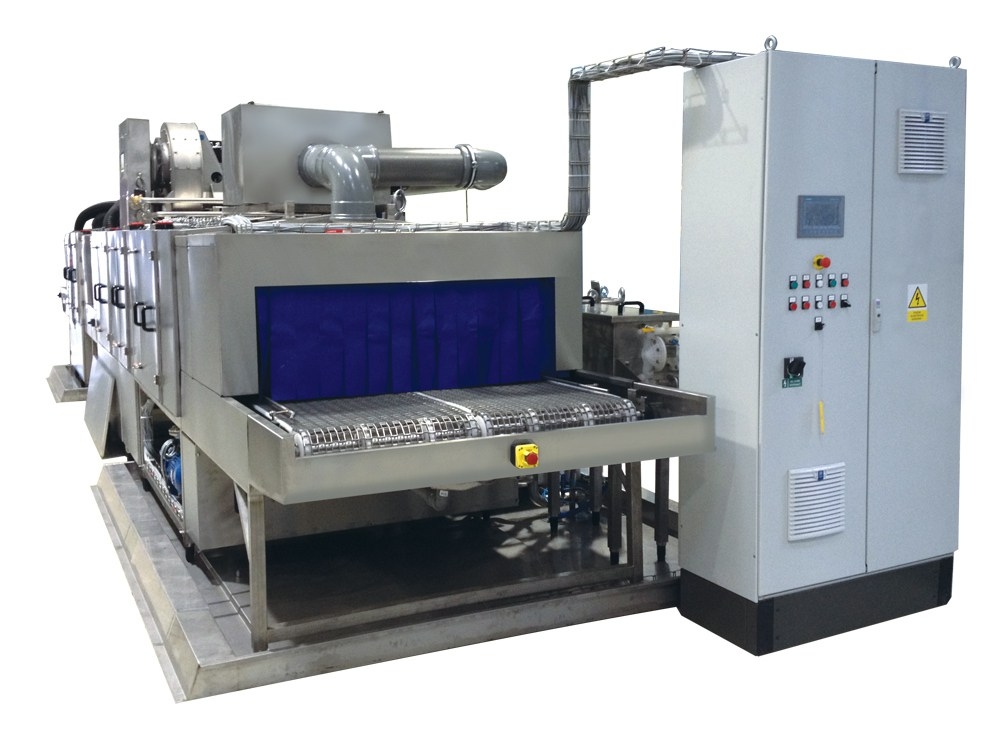
\includegraphics[height=2.5cm]{Fig/machine}
\hspace*{.2cm}
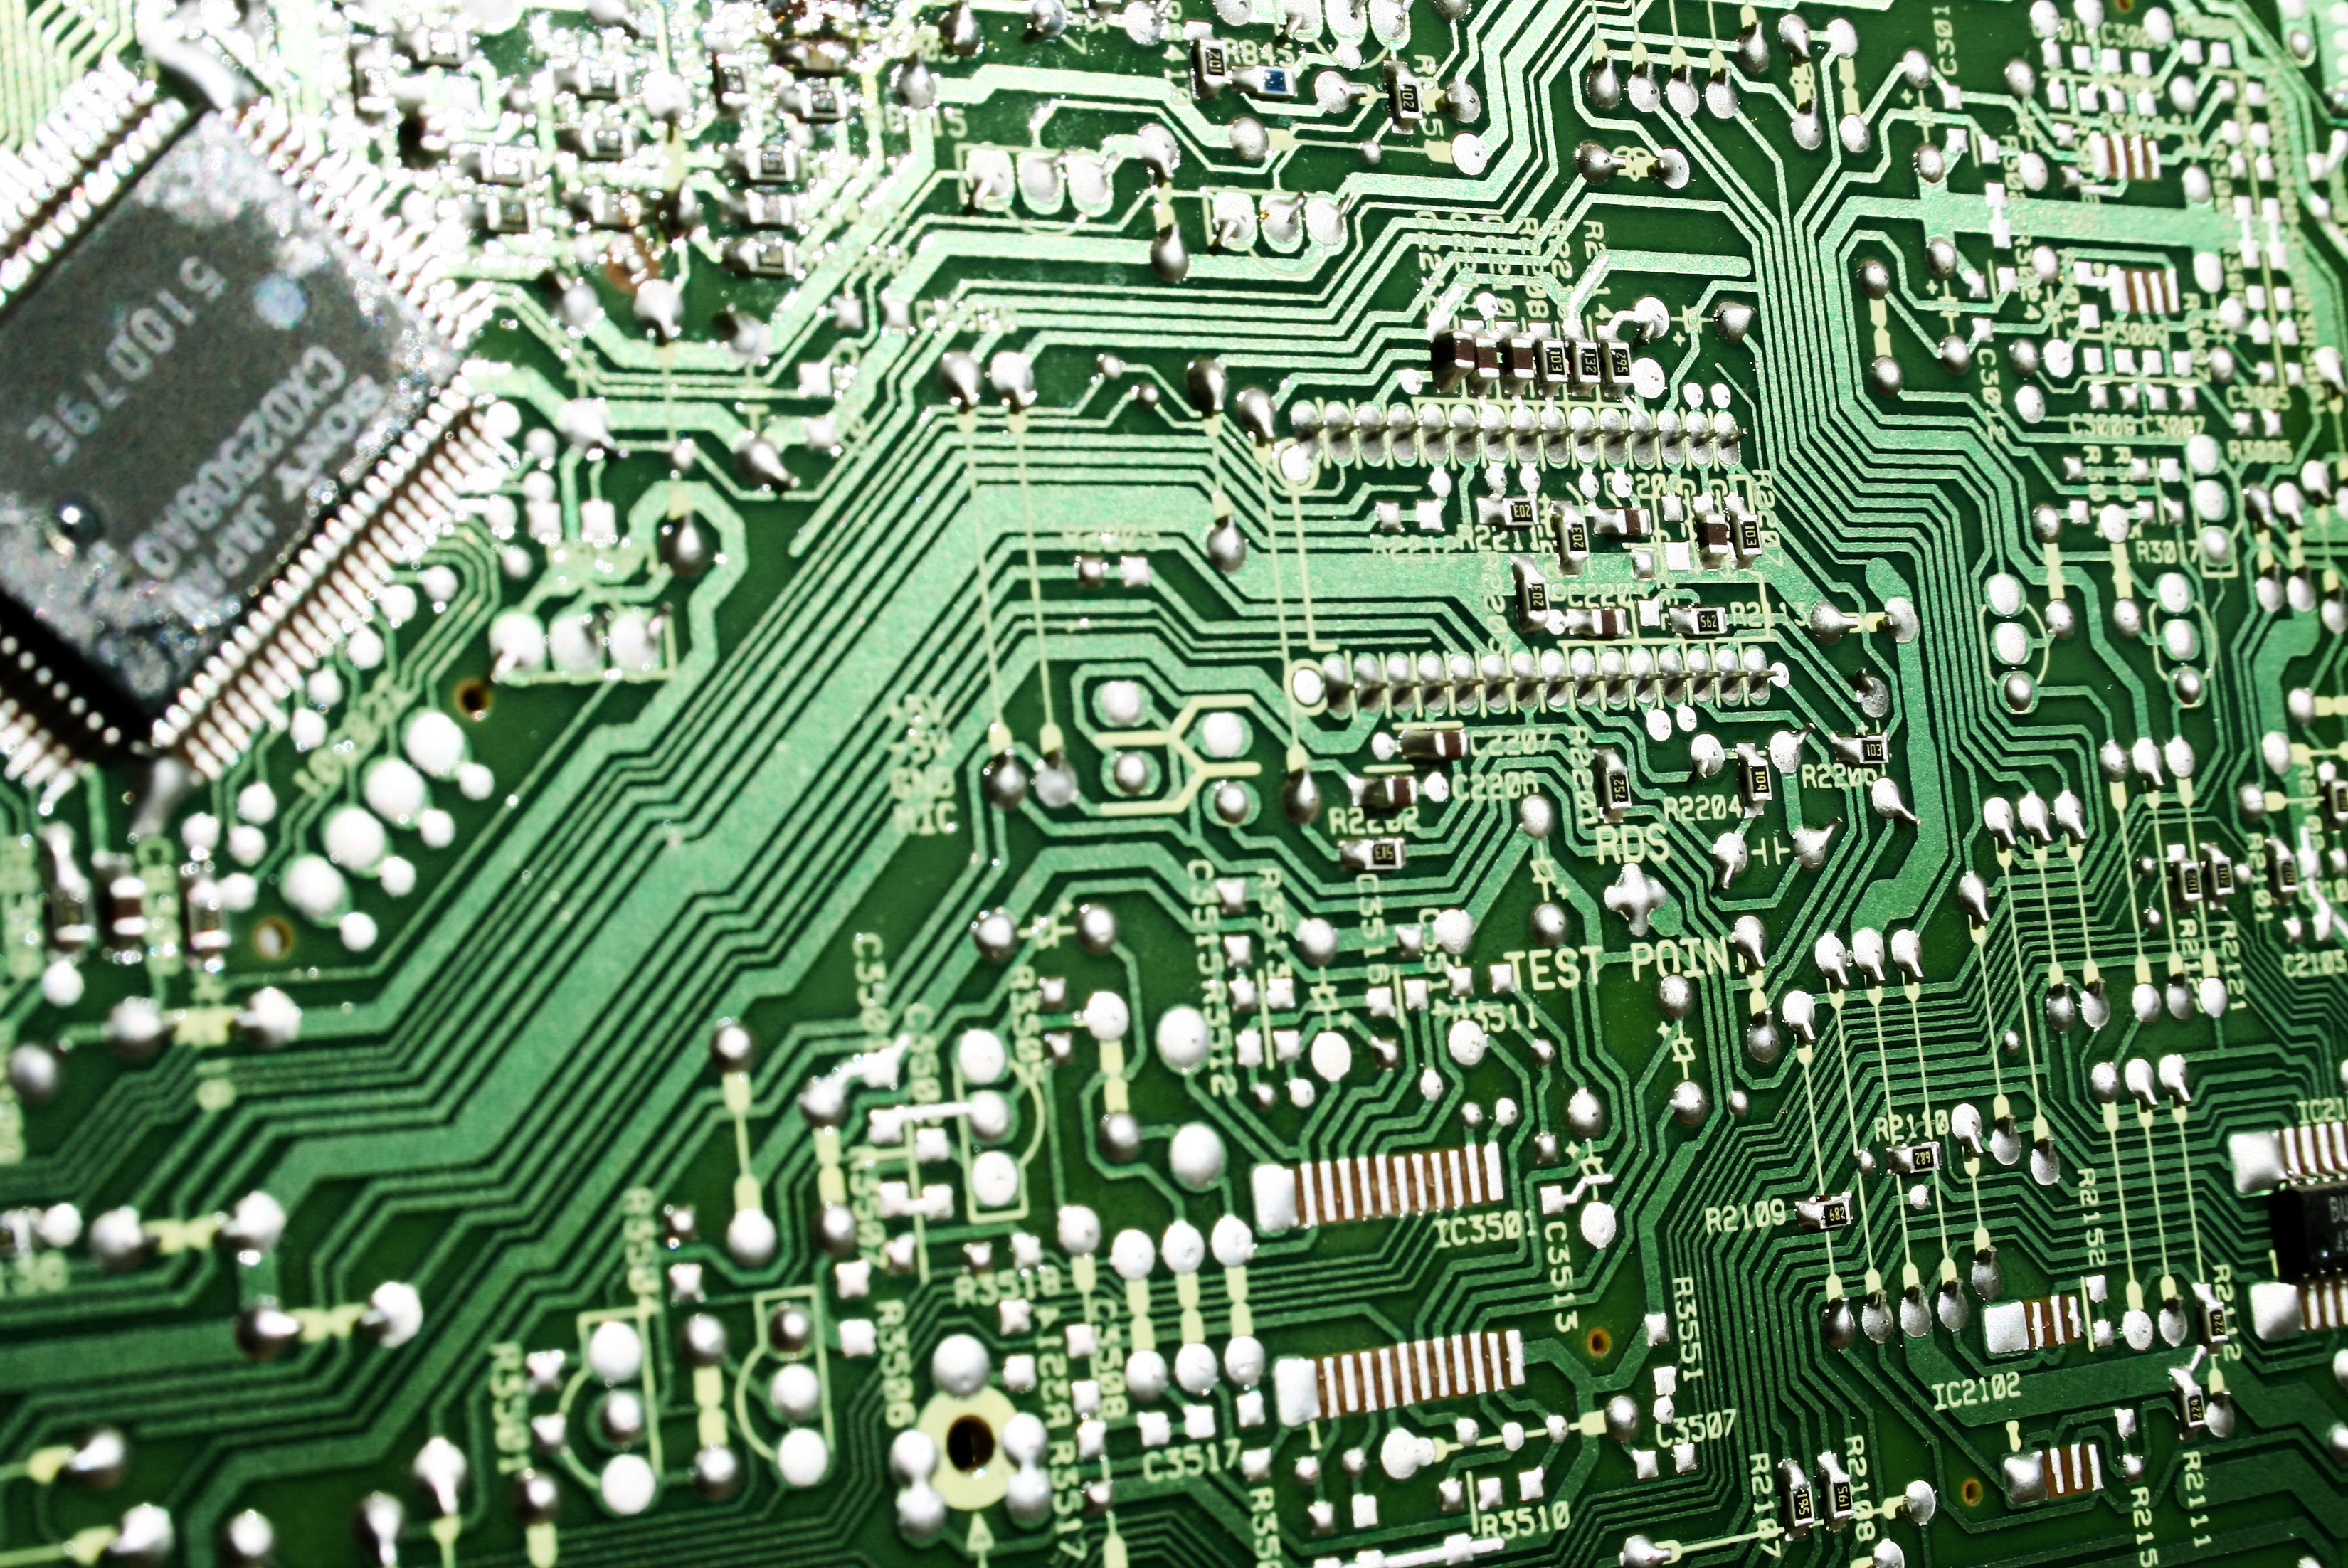
\includegraphics[height=2.5cm]{Fig/electronique}

programme \hspace{6em} contr{\^o}leur \hspace{6em} composante
\end{center}
\end{frame}

\begin{frame}{Un exemple : FlashFill}

\textcolor{red}{Programmation par l'exemple}, Gulwani (Microsoft Research) \\
\vskip1em
Inclus dans Microsoft Excel 2013

\begin{center}
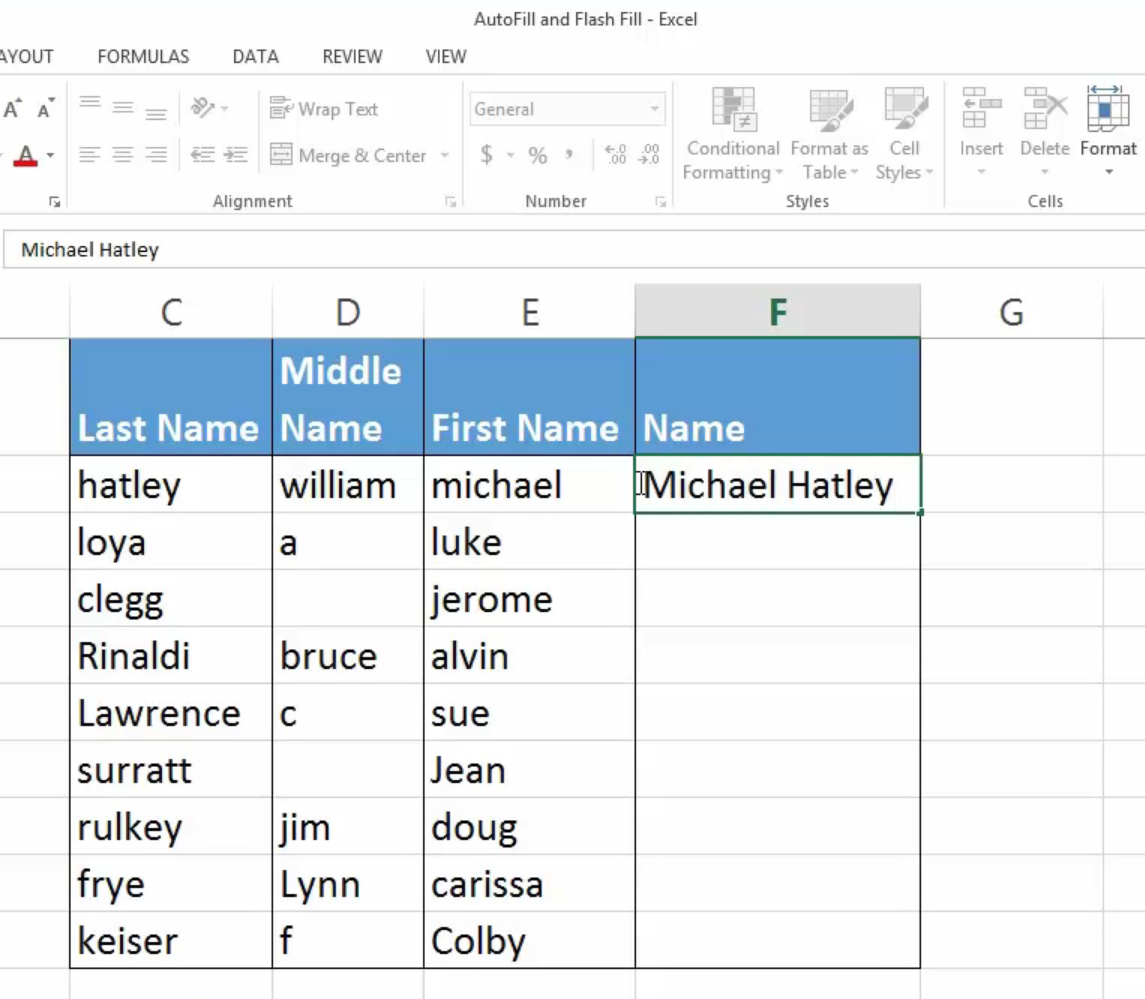
\includegraphics[height=4cm]{Fig/FlashFill}
\hspace*{.5cm}
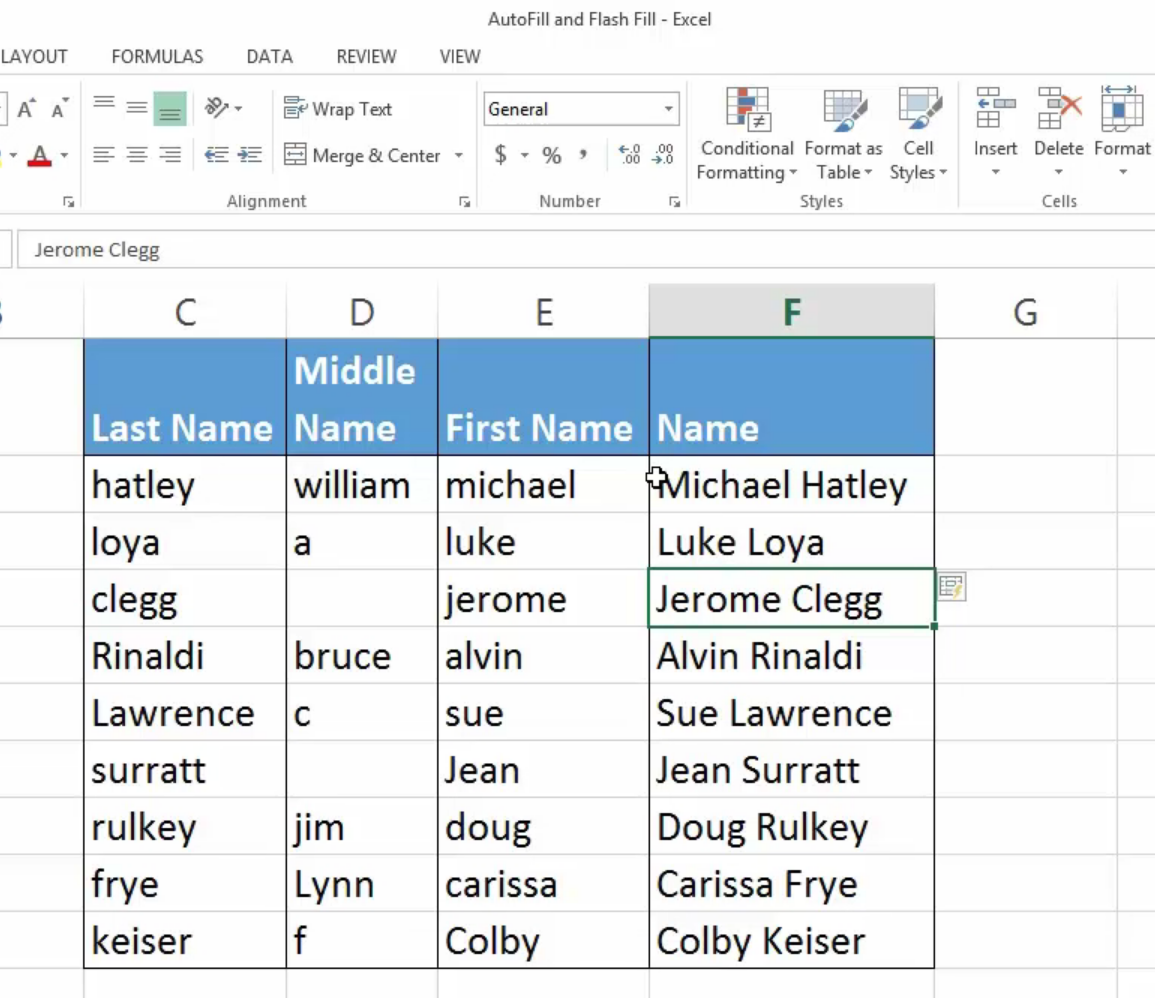
\includegraphics[height=4cm]{Fig/FlashFill2}
\end{center}

\textcolor{blue}{Correct d{\`e}s le premier essai dans 60\% des cas !}
\end{frame}

\begin{frame}{Synth{\`e}se : trois avantages}
\begin{itemize}
	\item \textcolor{red}{Certification} : un programme synth{\'e}tis{\'e} est (plus) facile {\`a} analyser (v{\'e}rification, explication)

	\vskip1em

	\item \textcolor{blue}{R{\'e}alisation} : exemple de la planification de mouvements en robotique (Rhoban)

\begin{center}
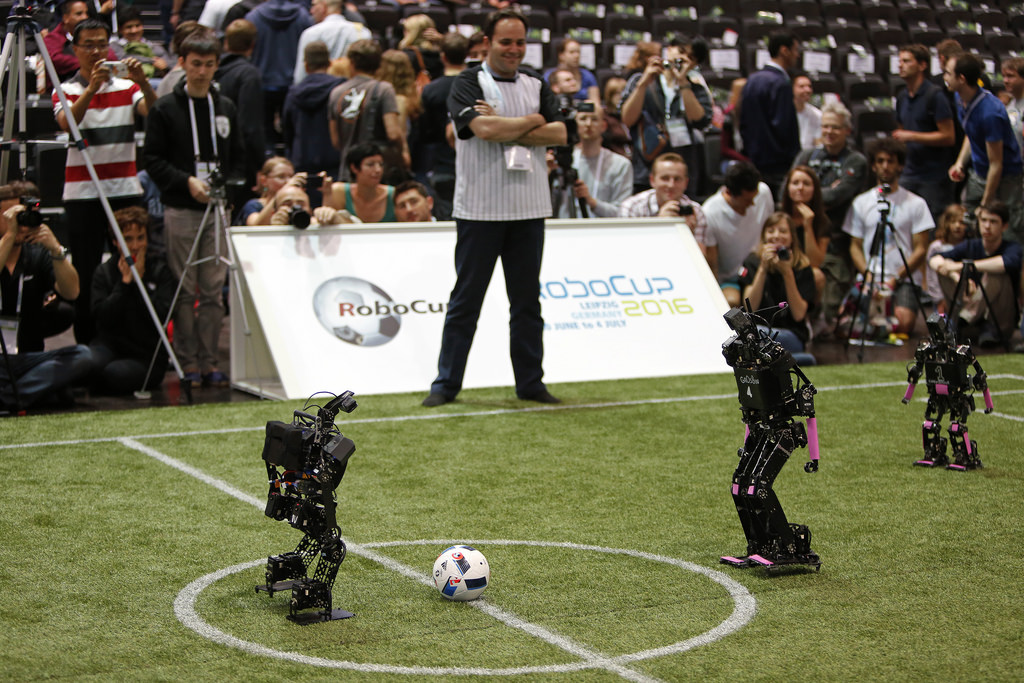
\includegraphics[height=2cm]{Fig/rhoban}
\end{center}

	\item \textcolor{magenta}{Sophistication} : exemple avec le jeu de Go (AlphaGo Zero, Google DeepMind)

\begin{center}
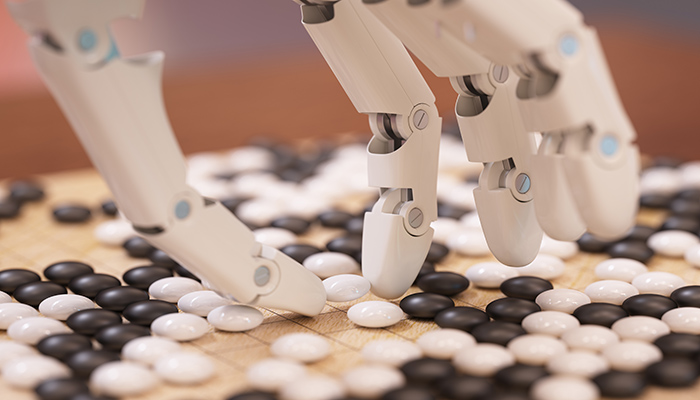
\includegraphics[height=2cm]{Fig/alphago}
\end{center}
\end{itemize}
\end{frame}

\begin{frame}{Synth{\`e}se : un inconv{\'e}nient}

Recherche d'un programme satisfaisant une sp{\'e}cification : \textcolor{magenta}{une aiguille dans une botte de foin} !
La synth{\`e}se est tr{\`e}s co{\^u}teuse en temps et en espace de calcul.
\vskip1em

\textit{Comment rendre la synth{\`e}se r{\'e}alisable en pratique ?}
\begin{framed}
\textbf{Approche du projet DeepSynth} : combiner \textcolor{red}{m{\'e}thodes formelles} et \textcolor{blue}{apprentissage} pour la synth{\`e}se
\end{framed}
\end{frame}

\begin{frame}{Combiner m{\'e}thodes formelles et apprentissage}
Source d'inspiration, papier fondateur :
\vskip1em

\begin{framed}
\textcolor{red}{DeepCoder}: Learning to Write Programs (ICLR 2017)
\end{framed}

\begin{itemize}
	\item \textcolor{blue}{Proof of concept} : combine m{\'e}thodes formelles et apprentissage profond pour la synth{\`e}se de programmes

\vskip1em

	\item \textcolor{purple}{D{\'e}passe largement} les approches purement bas{\'e}es sur les m{\'e}thodes formelles
	
\vskip1em

	\item D{\'e}montre (\textit{en pratique}) la capacit{\'e} des r{\'e}seaux de neurones {\`a} d{\'e}crire des \textcolor{magenta}{heuristiques}
\end{itemize}
\end{frame}

\begin{frame}{DeepSynthesis : une schizophr{\'e}nie th{\'e}matique}
\begin{itemize}
	\item \textcolor{red}{M{\'e}thodes formelles} : exact mais co{\^u}teux

	R{\'e}sultat r{\'e}cent : \textit{Quasipolynomial lower bounds for algorithms solving parity games}

	\vskip1em
	\item \textcolor{blue}{Apprentissage} : efficace mais approximatif

	R{\'e}sultat r{\'e}cent (collaboration au sein de l'institut Turing) : \textit{Data generation for programme synthesis}
\end{itemize}
\vskip1em

\begin{footnotesize}
\begin{itemize}
	\item \textbf{Bordeaux} : Hugo Gimbert, Laurent Simon, J{\'e}r{\'e}mie Bigot (IMB),
	\item \textbf{France} : Pierre Ohlmann (doctorant), Olivier Serre, Thomas Colcombet,
	\item \textbf{Institut Turing} : groupe ``fondations logiques des sciences des donn{\'e}es'',
	\item \textbf{Ailleurs} : {\L}ukasz Kaiser (Google Brain), Borja Balle (Amazon Cambridge), Bartek Klin (Varsovie), 
Jan K{\v r}et{\'i}nsk{\'y} (Munich), Marta Kwiatkowska (Oxford), Prakash Panangaden (Montr{\'e}al)
\end{itemize}
\end{footnotesize}
\end{frame}

\begin{frame}{D{\'e}roulement du projet DeepSynth}
\textbf{Deux axes}
\begin{itemize}
	\item \textcolor{red}{Jeux de parit{\'e}} : synth{\`e}se du $\mu$-calcul modal

	\textbf{Objectif} : \textit{Construire des algorithmes efficaces pour les jeux de parit{\'e} en s'appuyant sur des
m{\'e}thodes d'apprentissage}

	\item \textcolor{blue}{Processus de d{\'e}cisions markoviens} : syst{\`e}mes probabilistes,	base du reinforcement learning
	
	\textbf{Objectif} : \textit{{\'E}tudier la notion de strat{\'e}gie implantable}	
\end{itemize}

\vskip1em

\textbf{Calendrier}
\begin{itemize}
	\item \textbf{2019} : d{\'e}veloppements th{\'e}oriques et m{\'e}thodologiques,
	identification des potentielles applications

	\item \textbf{2020-2021} : embauche d'un post-doctorant pour travailler sur le premier axe,
	implantation des algorithmes et tests {\`a} diff{\'e}rentes {\'e}chelles
\end{itemize}
\end{frame}

\begin{frame}{Objectifs du financement}
\begin{itemize}
	\item \textbf{F{\'e}d{\'e}rer autour d'une discipline {\'e}mergente}
	\begin{enumerate}
		\item \textcolor{red}{Groupe de lecture} (commenc{\'e} en 2018)
		\item \textcolor{blue}{Recrutement d'un post-doctorant} et de stagiaires (M1,M2)
	\end{enumerate}

	\item \textbf{Rayonnement local}
	\begin{enumerate}
		\item \textcolor{olive}{Liens avec l'Institut Math{\'e}matiques de Bordeaux (IMB)}
		\item Organisation d'{\'e}v{\`e}nements ponctuels th{\'e}matiques (workshop, conf{\'e}rence)
		\item Contribuer au Bordeaux Artificial Intelligence Alliance (BAIA)
	\end{enumerate}

	\item \textbf{Visibilit{\'e} internationale}
	\begin{enumerate}
		\item Participation {\`a} des conf{\'e}rences internationales
		\item Visites {\`a} l'{\'e}tranger
		\item \textcolor{magenta}{Diffusion de vid{\'e}o-conf{\'e}rences de recherche en ligne}
		\item Blog de recherche (commenc{\'e} en 2018) \url{http://games-automata-play.github.io/}
		\item \textcolor{purple}{{\'E}dition et diffusion d'un ouvrage collaboratif sur la th{\'e}orie des jeux} (commenc{\'e} en 2018)
	\end{enumerate}

	\item \textbf{Pr{\'e}parer le d{\'e}p{\^o}t d'un projet europ{\'e}en (ERC)}
\end{itemize}
\end{frame}

\appendix

\begin{frame}
\textbf{Deux axes}
\begin{itemize}
	\item \textcolor{red}{Jeux de parit{\'e}} : synth{\`e}se du $\mu$-calcul modal

	\textbf{Objectif} : \textit{Construire des algorithmes efficaces pour les jeux de parit{\'e} en s'appuyant sur des
m{\'e}thodes d'apprentissage}

	\begin{itemize}
		\item 2019 : Notion de graphes universels (\textit{Thomas Colcombet, Pierre Ohlmann, Olivier Serre})

		\item 2020 - 2021 : Approche par les probl{\`e}mes de satisfaisabilit{\'e} (\textit{Laurent Simon, \underline{post-doctorant}})

		\item 2020 - 2021 : Approche par la programmation lin{\'e}aire
		(\textit{\underline{post-doctorant}})
	\end{itemize}

	\item \textcolor{blue}{Processus de d{\'e}cisions markoviens} : syst{\`e}mes probabilistes
	
	\textbf{Objectif} : \textit{{\'E}tudier la notion de strat{\'e}gie implantable}

		\begin{itemize}
		\item 2019 - 2020 : Algorithmes construisant des strat{\'e}gies implantables (\textit{Hugo Gimbert, Jan K{\v r}et{\'i}nsk{\'y}, Marta Kwiatkowska})

		\item 2020 - 2021 : Minimisation et approximation de processus (\textit{Pierre Ohlmann, Prakash Panangaden})
		
		\item 2020 - 2021 : Composition et d{\'e}compositions de processus (\textit{Bartek Klin})		

	\end{itemize}
\end{itemize}
\end{frame}

\begin{frame}

\begin{center}
\begin{tabular}{l|r}
& D{\'e}penses \\
\hline
Groupe de lecture (orateurs)
               & 10 000 \euro     \\
Stagiaires (x3, un par an)
               & 9 000  \euro     \\
Workshops et r{\'e}unions de projet (x3, un par an)
               & 25 000 \euro     \\
Missions (12 000 \euro\ par an)
               & 36 000 \euro     \\
Invit{\'e}s (x3, un ou deux mois chaque selon {\'e}volution)
               & 24 000 \euro     \\
Vid{\'e}o-conf{\'e}rences\footnote{Filmer et monter les communications : 1 000 \euro, deux {\'e}v{\`e}nements. Cr{\'e}er un MOOC, environ 20h de vid{\'e}os, 3 000 \euro.}
               & 5 000 \euro      \\
Soutien {\`a} la r{\'e}alisation de l'ouvrage collaboratif\footnote{Deux r{\'e}unions avec 15 auteurs. Reliquats : participation / organisation d'une {\'e}cole sur les jeux.}
			   & 30 000 \euro     \\
\hline
\textbf{Sous-total}
               & 139 000 \euro    \\
Charge administrative (8\%)
               & 11 120 \euro     \\
\hline
\textbf{Total}
               & 150 120 \euro    
\end{tabular}
\end{center}
\end{frame}

\end{document}
